\begin{figure*}
    \centering
    \begin{subfigure}{0.49\linewidth}
        \vspace*{-1ex}
        \centering
        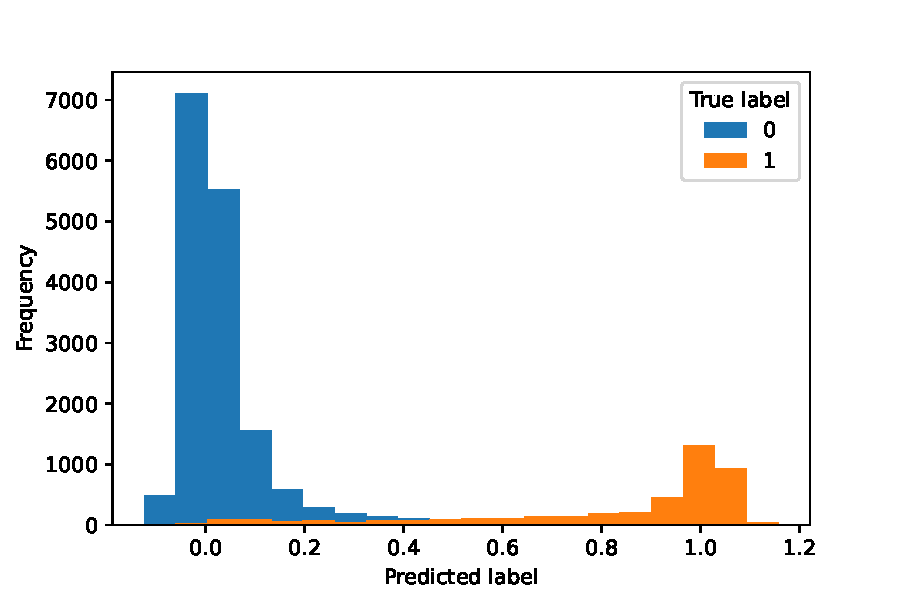
\includegraphics[width=\linewidth]{histogram-labels-bert-train.pdf}
        \vspace*{-3ex}
        \subcaption{Predictions with \BertBase on the training set.}
        \label{subfig:bert_train}
    \end{subfigure}
    \hfill
    \begin{subfigure}{0.49\linewidth}
        \vspace*{-1ex}
        \centering
        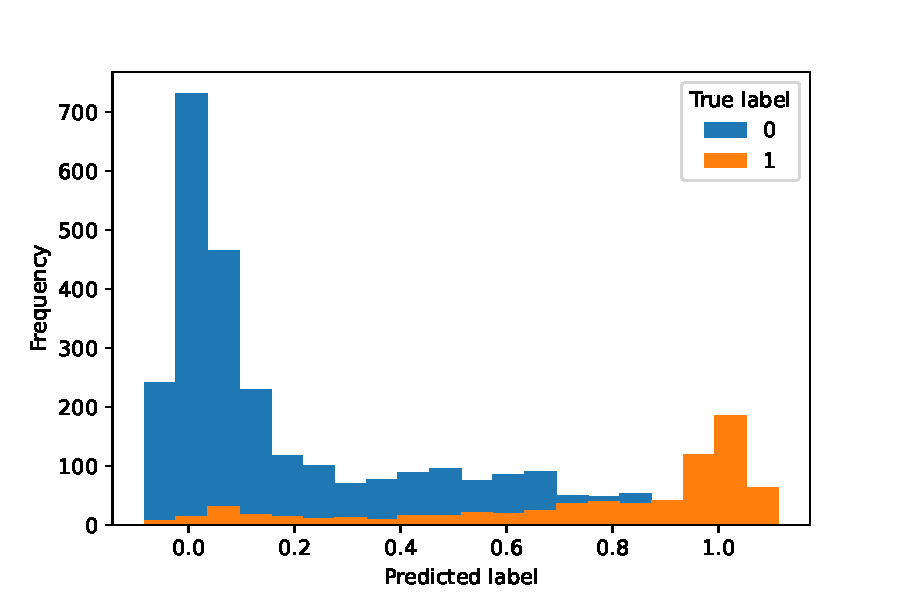
\includegraphics[width=\linewidth]{histogram-labels-bert-dev.pdf}
        \vspace*{-3ex}
        \subcaption{Predictions with \BertBase on the validation set.}
        \label{subfig:bert_dev}
    \end{subfigure}
    \begin{subfigure}{0.49\linewidth}
        \vspace*{-1ex}
        \centering
        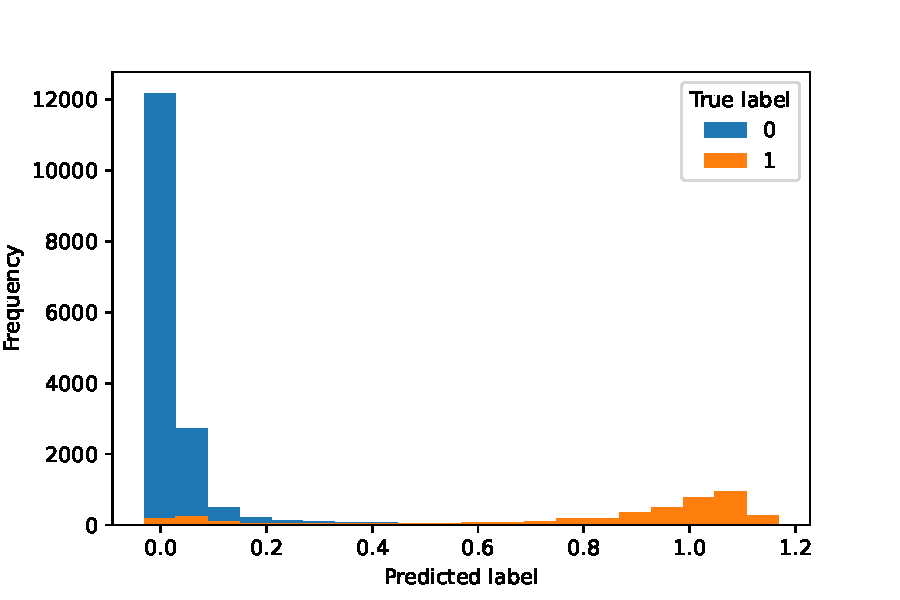
\includegraphics[width=\linewidth]{histogram-labels-roberta-train.pdf}
        \vspace*{-3ex}
        \subcaption{Predictions with \RobertaBase on the training set.}
        \label{subfig:roberta_train}
    \end{subfigure}
    \hfill
    \begin{subfigure}{0.49\linewidth}
        \vspace*{-1ex}
        \centering
        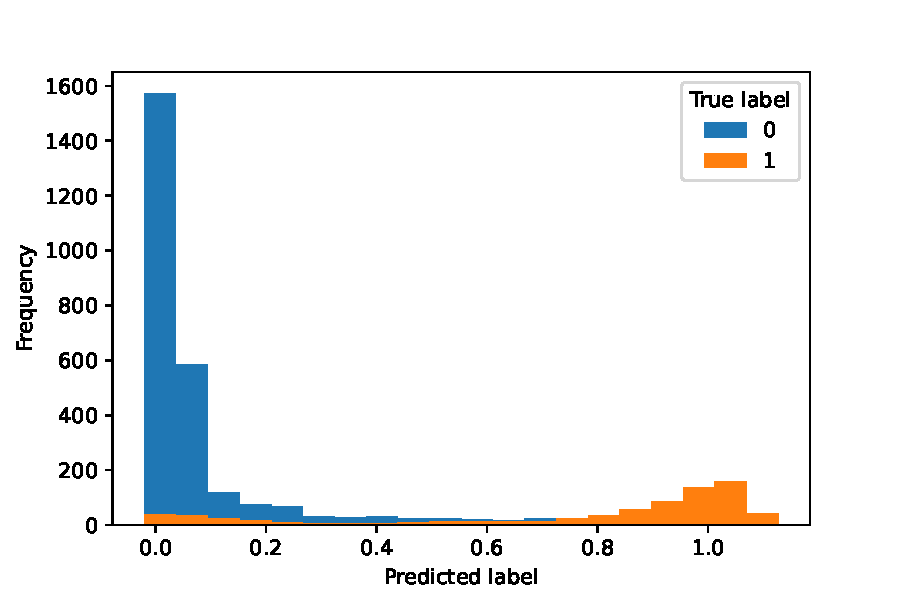
\includegraphics[width=\linewidth]{histogram-labels-roberta-dev.pdf}
        \vspace*{-3ex}
        \subcaption{Predictions with \RobertaBase on the validation set.}
        \label{subfig:roberta_dev}
    \end{subfigure}
    \caption{Histograms of predicted labels on the training and validation sets for argument key point pairs with the \BertBase and \RobertaBase classifiers. For good classifiers, predicted labels should approximately equal the true label~(0~or~1).}
    \label{fig:frequency}
\end{figure*}
